\chapter{DTLS}\label{chap:dtls}


\section{Overview}

DTLS (Datagram Transport Layer Security) is a protocol designed to communicate securely over UDP. It was first presented in \cite{modadugu2004design} by Modadugu and Rescorla as an adaptation of TLS for delay sensitive applications. The objective was to be as close as possible from TLS while working as secure over an unreliable transport protocol. Like TLS, this protocol operates at level 5 in the OSI model (session layer). Therefore, the operating system does not provide any support for the protocol and every application has to manage it by itself. Typically, it implies either reinventing the wheel or using an existing library such as OpenSSL\footnote{\url{https://www.openssl.org/}}.

The current version of this protocol is DTLS 1.2 described in RFC6347 \cite{rfc6347}. Our work is based on this version because no effort concerning a possible version 1.3 has been recently noticed. We may expect such a version will come after the discussions on TLS 1.3 that are taking place as we are writing these lines. For now, the suggested modifications have no impact on our current design as we explain in Section \ref{sec:tls13impact}.

Even if this protocol is standardized for some years, only few important applications are using it. In the open source world, OpenVPN has planned to use it when UDP is used. Unfortunately, it seems not to be a top priority and they are still using a homemade protocol to do TLS over UDP. For commercial applications, we have only heard about Cisco AnyConnect. It is a VPN client to be used with Cisco servers. Although the sources of AnyConnect are not available, a open source project is born from this application: OpenConnect\footnote{\url{http://www.infradead.org/ocserv/index.html}}.

Nevertheless, some people are working actively to make DTLS a default transport protocol when dealing with application level communications. More details about potential use cases are given in Section \ref{sec:dtls-usage}.

\subsection{Objectives}

Like TLS, DTLS has 3 strong requirements: authenticity, integrity and confidentiality.

\subsubsection{Authenticity}

We speak about authenticity when one host is able to verify that the messages are coming from another known host. Therefore, someone cannot pretend he is the sender of packets as the receiving host will detect it.

\subsubsection{Integrity}

The integrity is guaranteed if the information carried cannot be altered without being detected. As a consequence, someone between the communicating hosts cannot add, remove or modify a single bit without the hosts finding it out.


\subsubsection{Confidentiality}

Confidentiality assures that a non-authorized entity will not be able to extract an understandable content from a message. Thus, it is not sufficient to capture a conversation to get the information.

\section{Foundations}

In this section we present the way of working of DTLS and its roots. We will start with a reminder of TLS goals and principles since it is strongly related. Then, we will go through the major differences between these two protocols. Finally, we will list the steps of a typical connection and present the different messages involved.

\subsection{TLS}
\label{sec:tls}

TLS is a protocol designed to provide a secure connection over reliable transport. It takes place between a server and a client.

Once the channel is established :
\begin{itemize}
\item The client has authenticated the server (i.e. the server is really the one he pretends to be\footnote{Under the assumption that the certificates can be verified by a reliable certification authority. It is the role of the Public Key Infrastructure (PKI) to provide and verify the certificates.}) and optionally vice-versa.
\item All messages can only be read by the other host (an eavesdropping is possible but the clear text cannot be obtained)
\item The packets cannot be replayed or modified on the line without the host finding it out.
\end{itemize}

To achieve these points, cryptography is used between both hosts and the packets are authenticated. TLS authentication typically uses cryptographic signature based on public key together with a certification authority. During the handshake, the two hosts are negotiating which version of protocol will be used together with algorithms to encrypt and authenticate the future messages. Many algorithms can be used to exchange the keys over an insecure channel. The two most common algorithms for key exchange are RSA and Diffie-Hellman.

The first one suffers from a lack of the perfect forward secrecy property. As stated in \cite{diffie1992authentication}, the perfect forward secrecy is guaranteed if the disclosure of long-term secret keying material does not compromise the secrecy of the exchanged keys from earlier runs. In the case of RSA, if an attacker has recorded entirely some sessions and then discovers the server's private key, she is able to determine the symmetric keys used for every session. Moreover, in the discussions about the incoming TLS 1.3 standard, an agreement was reached to remove RSA key transport in this version\footnote{\url{https://www.ietf.org/mail-archive/web/tls/current/msg12266.html}}. Note that RSA can still be used to provide the digital signatures since they are only needed during a short moment and will not reveal information about the content itself if the keys are compromised.

An alternative to RSA is the Diffie-Hellman (DH) algorithm for key exchange described in \cite{diffie1976new}. The original approach used large prime numbers and the modular arithmetic to generate the master key. Nowadays, it is more common to use the elliptic curve approach since it allows to generate keys of smaller size than standard approach without decreasing the security level. In addition, to achieve perfect forward secrecy, the algorithms deal with ephemeral keys meaning that the DH parameters are different for every session. This leads to two well known algorithms : DHE (Diffie-Hellman ephemeral) and ECDHE (Elliptic Curve Diffie-Hellman ephemeral).

From this point, we will consider ECDHE for key exchange and RSA for signatures. Figure \ref{fig:tls_handshake} illustrates TLS handshake with this configuration. The figure is taken from Cloudfare, a CDN\footnote{Content Delivery Network} provider. The visitor is the client and Cloudfare could be any TLS ECDHE compatible server. 

\begin{figure}[!h]
\centering
\includegraphics[width=\linewidth]{images/ECDHEhandshake}
\caption[TLS handshake with ECDHE]{TLS handshake with ECDHE for key exchange (taken from \cite{tlsdhhandshake})}
\label{fig:tls_handshake}
\end{figure}

In the first phase, the client gives its version together with a list of algorithms for encryption and authentication called cipher suites. The client also gives to the server a random token to be used later. The server will then choose among the ones proposed: the version and the cipher suite to be used for the rest of the communication. A random server token is also included in the reply. In addition, the server may provide a session ID which can be used later for session resumption.

In a separated message, the server also provides its certificate to the client. It contains enough information for the latter to be able to verify server's identity. The certificate is generally emitted by a certification authority which is known by the client.

The next step comes with the server providing its DH parameters. In the case of ephemeral keys, the DH parameters must be different for every session. A digital signature using RSA with the server's private key is also included. The signature is computed not only on the information carried in this packet but also on all the previous exchanged messages. This is needed to prevent a man-in-the-middle attack. The genuine server is supposed to be the only one to hold the private key.

Then, the client provides its own DH parameters. Note that no signature is provided in this case as it is only optional to authenticate the client. Indeed, in some applications such as websites, this is not a requirement. After this step, both client and server can deduce the \textit{PreMasterSecret} and thus the master key with the random tokens exchanged before.

All messages following the handshake (containing application data) will be encrypted with symmetric cryptography using the keys deduced from the master key for this particular session. This will ensure the confidentiality. The two other objectives, authenticity and integrity of the messages, are ensured by a keyed-hash message authentication code (HMAC). It is generated as a hash on the content of the packet but the hash algorithm also integrates the secret key. Any cryptographic hash function can be used for this purpose but it is recommended to use at least \texttt{SHA256}. The choice of this function is also negotiated during the client hello, server hello phase. Even if it is better to first encrypt and then MAC the output as stated in \cite{bellare2000authenticated}, TLS works in reverse order for historical reasons. Currently people think it was a very bad idea from a security point of view and a RFC \cite{RFC7366} was published last year to push for the adoption of the encrypt-then-MAC technique on existing systems. It will probably be part of the TLS 1.3 RFC \cite{draft-tls13} to switch definitely to this better practice.

To prevent malicious replays disturbing the normal communication, TLS authenticates each packet with the associated sequence number. The sequence number is incremented for every packet sent but separately for each direction. Therefore each host has two counters: one for the packets sent and a second one for the packets received.

Thanks to a reliable transport protocol, these counters must never be transmitted explicitly because each host can compute them. As a consequence, if an attacker tries to replay packets, they will simply be rejected because the HMAC will not match with the most recent sequence number.

\subsection{Differences between TLS and DTLS}

\subsubsection{Unreliability}

The unreliability brought by UDP causes problems if we apply TLS over datagrams without any modification.

As we explain in the previous section, TLS uses implicit sequence numbers to authenticate packets. If a loss or a reordering occurs, then the sequence number considered by the receiving host will be wrong and the integrity check will fail. To solve this problem, DTLS modifies the record layer and adds a new field to carry the sequence number in every packet. The DTLS 1.2 record layer is presented on Listing \ref{lst:dtls-record}.

\addtypes{ContentType, ProtocolVersion, uint16, uint48, opaque}
\begin{lstlisting}[caption=DTLS record layer, label=lst:dtls-record]
struct {
   ContentType type;
   ProtocolVersion version;
   uint16 epoch;                                    // New field
   uint48 sequence_number;                          // New field
   uint16 length;
   opaque fragment[DTLSPlaintext.length];
 } DTLSPlaintext;
\end{lstlisting}


Epoch is used by endpoints to identify the keys used to protect the payload. The epoch is incremented by one once a \texttt{changeCipherSpec} is sent. Initially, the epoch is set to 0 for the handshake and the following \texttt{changeCipherSpec} will be the first message being part of the next epoch. The sequence number is set back to 0 once a new epoch has started. Due to the risks of retransmission or reordering, the endpoint need a way to know which set of keys were used to crypt the payload, because it cannot simply assume it is the latest negotiated keys. This need is fulfilled thanks to the epoch field.

Another problem raised by unreliability is the fact that in TLS the handshake has to follow a particular order and if not the connection is simply aborted. This is clearly incompatible with losses and retransmissions. To handle potential losses in the handshake phase, implementation must retransmit the last packet after a given time if no answer has been received from the other host (see \cite{rfc6347} Section 4.2.4).

To deal with possible reordering, all handshake messages have a given sequence number. So if a message is received before another one, the first message must be queued for further processing.

\subsubsection{Messages size}

The message size is a potential issue because TLS (and thus DTLS) messages can be as large as $2^{24}-1$ bytes while UDP datagrams are often limited to $1500$ bytes. Therefore, each DTLS handshake message may be fragmented over several DTLS records and then rebuilt. One fragment must fit in a single IP datagram to avoid IP fragmentation.

The benefits to this requirement are stated in the original DTLS paper \cite{modadugu2004design} :
\begin{itemize}
\item The DTLS layer does not need to buffer partial records, host memory can be used more efficiently.
\item It is quite possible that datagrams carrying the remaining record fragments are lost, in which case the received fragments are useless and cannot be processed.
\item Buffering record fragments would unnecessarily complicate a DTLS implementation without providing any obvious benefit.
\end{itemize}

Note that even if IP fragmentation occurs, DTLS will still operate correctly on top of re-assembly since it is transparently handled by the kernel.

The TLS handshake message is modified as shown on Listing \ref{lst:dtls-handshake}. The handshake message following this structure is also encapsulated into the record layer presented on Listing \ref{lst:dtls-record}.

\addtypes{HandshakeType, uint16, uint24, case, select}
\begin{lstlisting}[caption=DTLS handshake message, label=lst:dtls-handshake]
   struct {
     HandshakeType msg_type;
     uint24 length;
     uint16 message_seq;                               // New field
     uint24 fragment_offset;                           // New field
     uint24 fragment_length;                           // New field
     select (HandshakeType) {
       case hello_request: HelloRequest;
       case client_hello:  ClientHello;
       case hello_verify_request: HelloVerifyRequest;  // New type
       case server_hello:  ServerHello;
       case certificate:Certificate;
       case server_key_exchange: ServerKeyExchange;
       case certificate_request: CertificateRequest;
       case server_hello_done:ServerHelloDone;
       case certificate_verify:  CertificateVerify;
       case client_key_exchange: ClientKeyExchange;
       case finished: Finished;
     } body;
   } Handshake;
\end{lstlisting}

\subsubsection{Anti-Replay strategy}

In TLS, sequence numbers follow sequentially and a packet cannot be replayed because the HMAC verification will fail immediately. Such a drastic solution cannot be applied in DTLS because reordering or losses may occur. The DTLS 1.2 RFC \cite{rfc6347} sec. 4.1.2.6 describes the procedure to avoid replay using a sliding window. This strategy considers packets as valid even if they have been delayed or reordered while they are relatively close from the latest packets received. At the same time, the implementation must remember the packets received inside the sliding window and silently discard the replayed packets. Therefore, the MAC verification will only be done if the packets have not been received before, otherwise an undesirable packet is discarded at the record layer stage.

\subsubsection{Anti-DoS for the handshake}

In order to prevent DoS (Denial of Service) attacks, DTLS adds an additional step in comparison with the TLS handshake. Indeed, an attacker could send a lot of \texttt{ClientHello} messages and the server will have to keep a state for each of them, rapidly increasing the memory needed. Instead, the first \texttt{ClientHello} will not directly trigger a \texttt{ServerHello} but a \texttt{HelloVerifyRequest}. This message only carries the protocol version and a cookie as presented in Listing \ref{lst:dtls-helloverify}. This cookie must be retransmitted in the next Client Hello message. As we can seen on Listing \ref{lst:dtls-clienthello}, a new field has effectively been added to the \texttt{ClientHello} message.

\addtypes{ProtocolVersion, opaque}
\begin{lstlisting}[caption=DTLS HelloVerifyRequest message, label=lst:dtls-helloverify]
struct {
 ProtocolVersion server_version;
 opaque cookie<0..2^8-1>;
} HelloVerifyRequest;
\end{lstlisting}


\addtypes{ProtocolVersion, opaque, Random, SessionID, CipherSuite, CompressionMethod}
\begin{lstlisting}[caption=DTLS ClientHello adapted message, label=lst:dtls-clienthello]
struct {
 ProtocolVersion client_version;
 Random random;
 SessionID session_id;
 opaque cookie<0..2^8-1>;                             // New field
 CipherSuite cipher_suites<2..2^16-1>;
 CompressionMethod compression_methods<1..2^8-1>;
} ClientHello;
\end{lstlisting}

The additional \texttt{HelloVerifyRequest} message is also a counter measure against amplification attacks. Such attacks are trying to redirect traffic to overload a particular target by using an other server to generate bigger messages. These attacks are possible if the generated message is larger than the one triggering it. It is the case with DNS since the reply is larger than the request if a particular domain has multiple DNS records. It becomes then a vector for DoS attacks (see Figure \ref{fig:amp_attack} taken from \cite{dns-amp}).


\begin{figure}[!ht]
\centering
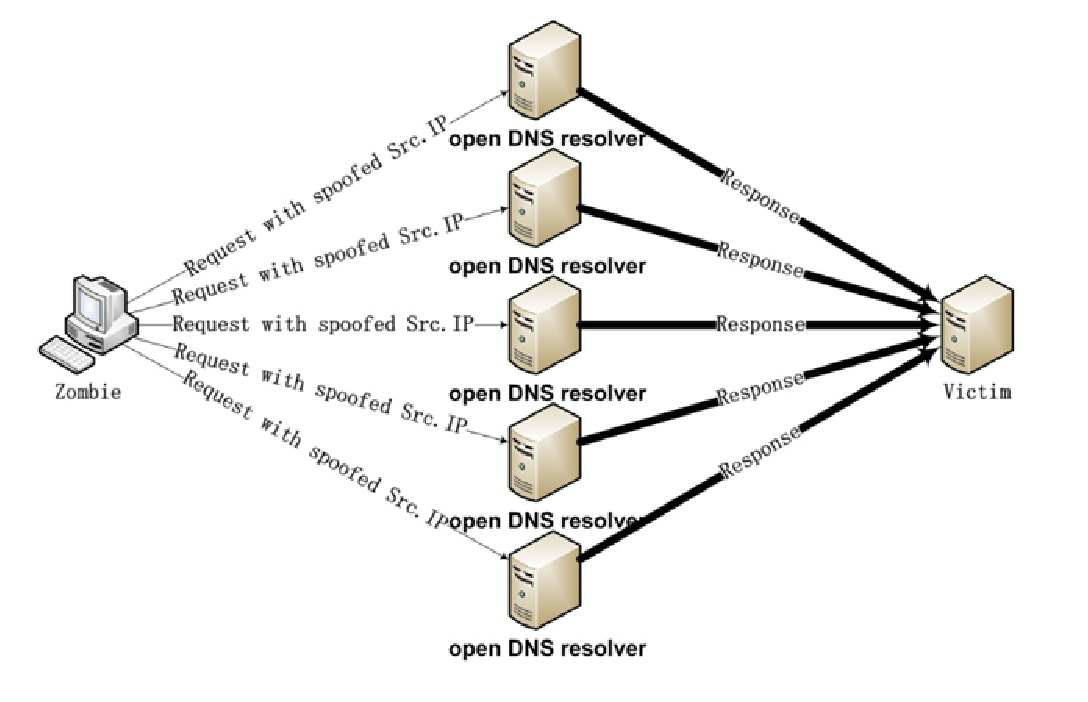
\includegraphics[width=\textwidth]{images/amplificationattacks}
\caption{Example of amplification attack with DNS}
\label{fig:amp_attack}
\end{figure}

For DTLS, the \texttt{ServerHello} is not larger than the \texttt{ClientHello} but amplification attack could still be possible (without the \texttt{HelloVerifyRequest}). Indeed, other messages are sent together with the \texttt{ServerHello}, including the one carrying the certificate (that could be quite large). Therefore, the additional step introduced with the \texttt{HelloVerifyRequest} (which is relatively small) prevents this kind of attack because the client has to prove it can answer at this address.

When the client sends its first \texttt{ClientHello}, the cookie field is initially empty. The server will then generate a new cookie which allows for a stateless exchange. It sends the \texttt{HelloVerifyRequest} with the cookie and doesn't remember anything about the client\footnote{This is indeed an exception to the retransmission measures. A \texttt{HelloVerifyRequest} will never be retransmitted, the client must first send another \texttt{ClientHello}.}. The DTLS server must generate cookies in such a way that they can be verified without retaining any per-client state on the server. A way to compute it is given in the RFC6347 section 4.2 \cite{rfc6347}:

\begin{lstlisting}
Cookie = HMAC(Secret, Client-IP, Client-Parameters)
\end{lstlisting}

The \texttt{Secret} is random and generated by the server. It could be periodically refreshed to invalidate previous cookies. Once a \texttt{ClientHello} has been received with a cookie, the server recomputes it and if both match, the connection can continue as in TLS with a \texttt{ServerHello} message.

\section{Typical DTLS communication}

\subsection{Handshake}

\begin{figure}[!h]
\centering
\begin{msc}[r]{DTLS Handshake}

\setlength{\instfootheight}{0em}
\setlength{\instheadheight}{0em}
\setlength{\instdist}{0.7\linewidth}
\setlength{\levelheight}{3em}

\declinst{client}{Client}{}
\declinst{server}{Server}{}

\mess{Client Hello}[t]{client}[0.3]{server}[1]
\nextlevel
\mess{Hello Verify Request}[t]{server}[0.3]{client}[1]
\nextlevel
\mess{Client Hello (w/ cookie)}[t]{client}[0.3]{server}[1]
\nextlevel
\mess{Server Hello}[t]{server}[0.5]{client}[1]
\nextlevel
\mess{Certificate}[t]{server}[0.5]{client}[1]
\nextlevel
\mess{Server Key Exchange}[t]{server}[0.5]{client}[1]
\nextlevel
\mess{Server Hello Done}[t]{server}[0.3]{client}[1]
\nextlevel
\mess{Client Key Exchange}[t]{client}[0.3]{server}[1]
\nextlevel
\mess{Change Cipher Spec}[t]{client}[0.3]{server}[1]
\nextlevel
\mess{Change Cipher Spec}[t]{server}[0.3]{client}[1]
\nextlevel
\nextlevel
\end{msc}
\caption{DTLS handshake with ECDHE-RSA cipher suite}
\label{fig:dtls-handshake}
\end{figure}


Figure \ref{fig:dtls-handshake} depicts a typical handshake with authentication of the server only and the ECDHE-RSA cipher suite\footnote{It means that Elliptic Curve Diffie-Hellman ephemeral is used for the key exchange and RSA for the signature.}. All messages before the \texttt{ChangeCipherSpec} are part of epoch 0. Their role is to negotiate the algorithms that will be used to compute the master key. The \texttt{Client Hello} has also the role to carry potential extensions supported by the client. If the server supports them as well, it will include them in the following \texttt{Server Hello} message. This is also where we chose to advertise our MPDTLS extension as explained in Chapter \ref{chap:design}.

The only difference with TLS (Section \ref{sec:tls}) is the presence of a second \texttt{ClientHello}. The first one is sent with no cookie and the second one must repeat the cookie received with the \texttt{HelloVerifyRequest}. Then the server confirms the cipher suite to be used through the \texttt{ServerHello} and directly sends its certificate and its ephemeral public key\footnote{In the case of ECDHE, it consists of the public DH parameters. Namely the domain parameters to define a particular curve.} including a signature of all previous exchanged messages. Finally the server sends the \texttt{ServerHelloDone} to explicitly say that the handshake is finished on its side.

Thereafter the client must also send its DH ephemeral public key. At this point, both parties have all the elements in their hands to compute the premaster secret. Note that unlike RSA, the secret is never communicated through the channel. With the random information exchanged through the \texttt{ClientHello} and \texttt{ServerHello}, each host can also compute the master key on its side. Consequently each peer will use this key to derive the set of keys used to communicate in the next epoch. The first messages of epoch 1 are the \texttt{ChangeCipherSpec} messages. They explicitly mark the separation between the handshake and the rest of the communication. Even if they are technically separated from the handshake, they are still considered as being part of it from a conceptual point of view.


\subsection{Application data}

Once the handshake has been completed, the peers can exchange Application Data packets. They are first encrypted and authenticated using the parameters negotiated earlier, then encapsulated into a Record Layer (Listing \ref{lst:dtls-record}).

DTLS doesn't bring any additional guarantee concerning the reliability of the link. As shown in Figure \ref{fig:dtls-data}, packets may be lost on the way and the application must deal with it. The sequence number for each message is indicated between chevrons. Sequence numbers are carried in clear inside the record layer, so each host knows how to verify the MAC and authenticate the packet.

\begin{figure}[!h]
\centering
\begin{msc}[r]{DTLS communication}

\setlength{\instfootheight}{0em}
\setlength{\instheadheight}{0em}
\setlength{\instdist}{0.7\linewidth}
\setlength{\levelheight}{3em}

\declinst{client}{Client}{}
\declinst{server}{Server}{}

\mess{Application Data <1>}[t]{client}[0.3]{server}[1]
\nextlevel
\mess{Application Data <1>}[t]{server}[0.3]{client}[1]
\nextlevel
\nextlevel
\lost[r]{Application Data<2>}[t]{}{client}[3]
\nextlevel
\mess{Application Data<3>}[t]{client}[0.3]{server}[1]
\nextlevel
\mess{Application Data<2>}[t]{server}[0.5]{client}[1]
\nextlevel
\nextlevel
\end{msc}
\caption{DTLS application data exchange}
\label{fig:dtls-data}
\end{figure}

\section{Use cases}

\label{sec:dtls-usage}

DTLS can be used almost everywhere UDP is used. We can think about applications such as VoIP (Voice over IP), multimedia, online gaming. Every application that wants to secure its communication but still benefit from faster transmission time of UDP may take advantage of using DTLS.

Of course the application has to cope with losses or reordering, but this is already the case for real time communication. As regards telephony, blank sounds replace the missing packets. For online gaming, high speed communication between the server and the client is needed to determine the character's position for instance. But if one packet is lost, the position can be determined by the next packet and the application will not be disturbed.

For video streaming applications, techniques are used to introduce a slight redundancy at the codec level in such a way that if some packets are lost, one frame may be missing but at least the video is still watchable\footnote{Of course, the application must a use a proper codec and compression method.}. It is also possible to introduce a small buffer to handle reordering.

In a recent Internet draft \cite{dtls-as-subtransport}, companies are trying to make DTLS the default sub-transport protocol for all application-level protocols when security is needed. This will raise DTLS to the rank of "good practice" for secured communications.

Another important use case for DTLS comes with its integration in WebRTC\footnote{\url{http://www.webrtc.org/}}. This is an open project which has an objective to bring real time communications to browsers and mobile applications via simple APIs. In this context, DTLS has been chosen to ensure the communication between two peers (i.e. browsers or mobile apps). The internet draft describing the security architecture of WebRTC \cite{ietf-rtcweb-security-arch} proposes to use SRTP over DTLS for multimedia communications and DTLS alone for any other kind of data. Figure \ref{fig:webrtc} is taken from a presentation \cite{rescorla2011proposed} made by E.Rescorla and shows how the connection is set up in this proposed design.  

\begin{figure}[!ht]
\centering
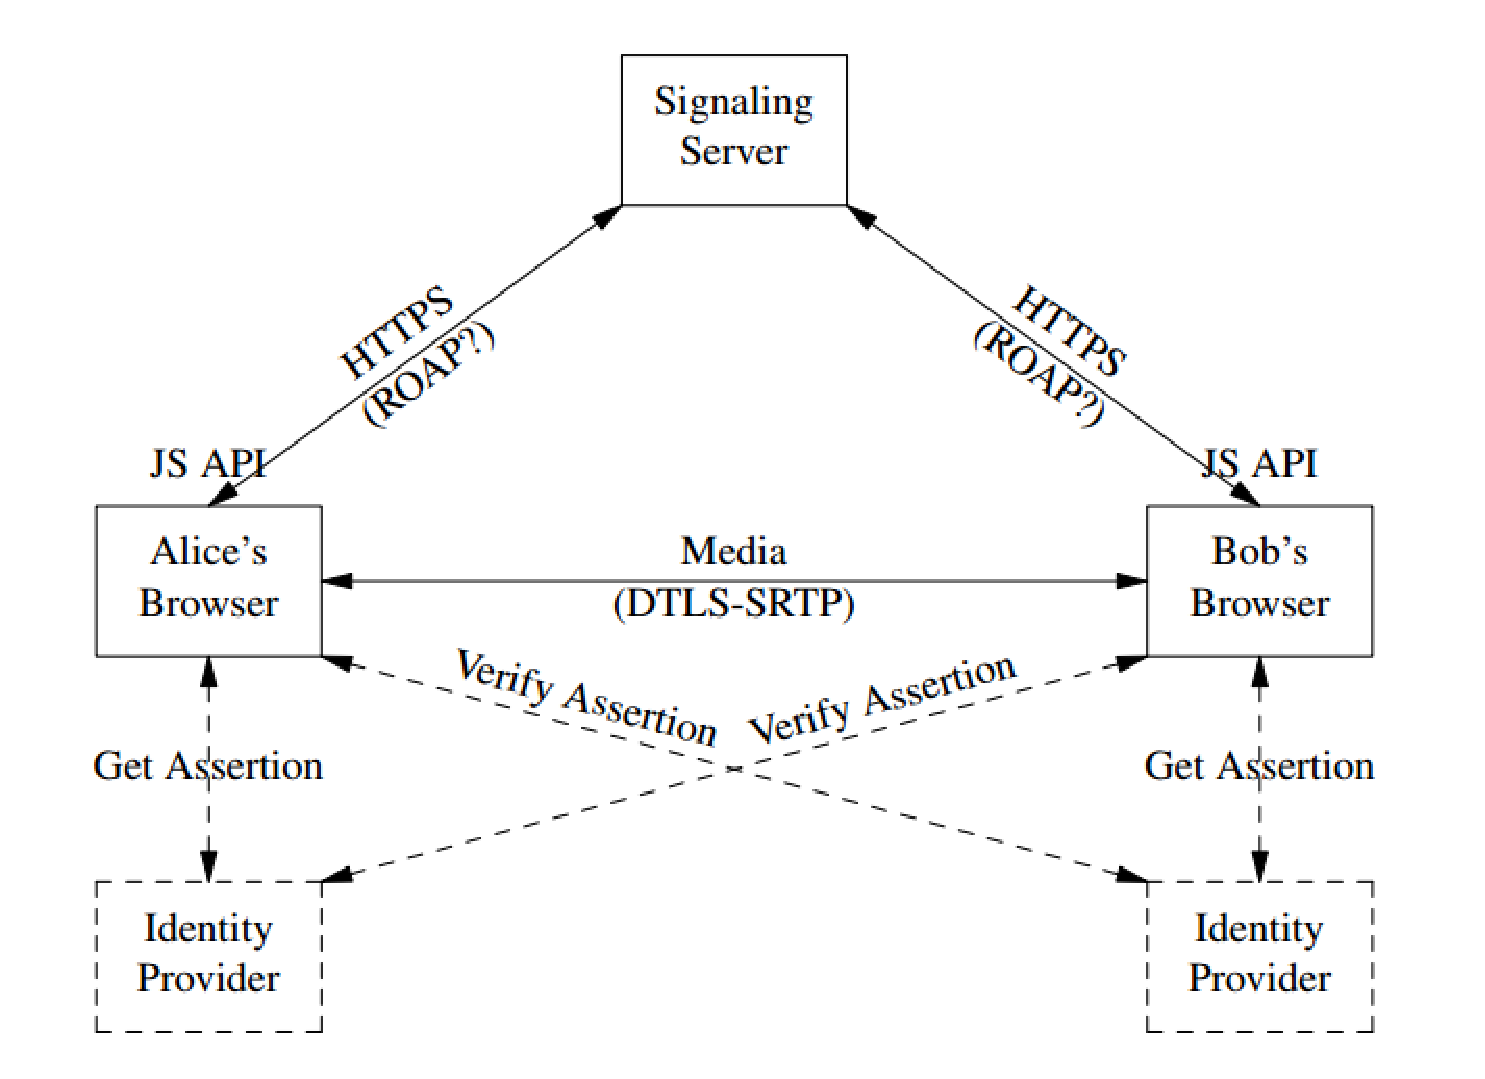
\includegraphics[width=0.9\textwidth]{images/webrtc.eps}
\caption{Proposed design for WebRTC security architecture}
\label{fig:webrtc}
\end{figure}

By the peer to peer nature of this application, a signalling server is needed to act as a "rendez-vous" point and to perform NAT traversal. Then the handshake can take place and identity providers issue and verify certificates. Finally all data are transmitted through the DTLS transmission and multiple SRTP sessions can use the same DTLS session. 

To sum up, all these applications may benefit from using DTLS but also MPDTLS as it will allow more resilience and better performances. We will demonstrate this point in the following chapters.

\section{Security considerations}
\label{sec:tls-sec}

Most of the security considerations are the same as those of TLS 1.2 \cite{RFC5246} since DTLS is only an adaptation of TLS for unreliable transport protocols.

The attacks known for TLS could theoretically be used for DTLS as well. This is the case for the "secure renegotiation". As a reminder, this vulnerability allows an attacker who can hijack a HTTPS connection to add custom request to a communication between the client and the web server. Even if the attacker cannot retrieve the content of the communication, it can still have dramatic consequences. As depicted on Figure \ref{fig:tls-reneg} taken from \cite{tls-reneg}, an attacker can inject bank orders and then trigger the renegotiation with a real client. The bank order is only delayed and when the renegotiation is completed, it is executed before anything else. The best solution up to know is to disable by default this feature on servers. \todo{Or to implement the extension RFC5746}

\begin{figure}[!ht]
\centering
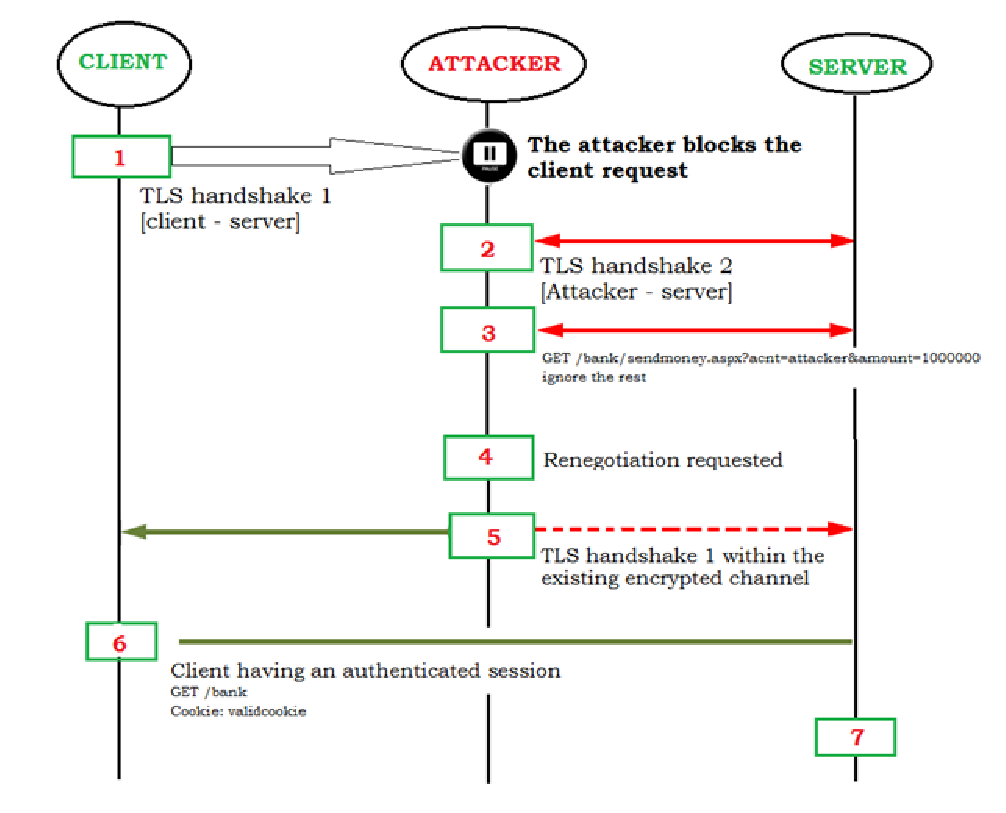
\includegraphics[width=0.8\textwidth]{images/TLSrenegotiation}
\caption{TLS renegotiation vulnerability}
\label{fig:tls-reneg}
\end{figure}

Other attacks could also be applied to DTLS and be more efficient on DTLS than on TLS, namely the DoS attacks. Two main categories can be identified :

\begin{itemize}
\item The blind DoS : packets are being transmitted with a spoofed IP address to redirect the traffic to another target (amplification attack) or to simply not diclose the IP address of the attacker. They are called blind because the attacker will never receive any answer from the server. They are made easier with UDP because no handshake is needed with the server.
\item Computational DoS : the attacker can reply to certain messages but will try to optimize the ratio between the work he has to do and the work he is asking to the server.
\end{itemize}

Blind DoS are made impossible in TLS because the attacker must first complete the TCP handshake and thus prove he can answer at this address. As presented earlier, the introduction of the \texttt{Hello Verify Request} will prevent this kind of attack for DTLS too.  Although it is not a strict requirement to implement this feature in DTLS (\cite{rfc6347} Section 5), it is strongly recommended for DTLS servers  unless there is a good reason to think that no amplification is possible in their environment.

Nevertheless the second type can still be used to disturb a server running DTLS or even TLS. As explained by E. Rescorla in \cite{tls-dos}, nothing is done at the design level to prevent these kind of attacks because it would imply putting a lot of work on the client side. It is generally a bad idea for performances. Moreover, the attackers are often using infected computers of casual people to launch DoS attacks. Therefore they have a lot of CPU power available anyway.

\section{Heartbeat extension}

The heartbeat extension is unfortunately known for the famous heartbleed bug\footnote{\url{http://heartbleed.com/}} detected in April 2014. Every server using OpenSSL at this time was vulnerable and part of the memory could be retrieved (including private keys, passwords\dots). It is important to note that the error came from the implementation of the extension inside OpenSSL and not from the standard itself.

Anyway, this extension can be really useful to assess the availability of a link and also provides a keep-alive feature. It is quite simple but it also allows for extensibility and new messages as stated in RFC6520 \cite{rfc6520}. The structure of a heartbeat message is presented on Listing \ref{lst:hb-msg}. This will take place on top of the Record Layer (Listing \ref{lst:dtls-record}). The advertisement of this extension is made through a Hello extension. It also defines the behavior of the hosts upon the reception of Heartbeat messages.

\addtypes{HeartbeatMessageType}
\begin{lstlisting}[caption=Heartbeat message, label=lst:hb-msg]
struct {
  HeartbeatMessageType type;
  uint16 payload_length;
  opaque payload[HeartbeatMessage.payload_length];
  opaque padding[padding_length];
} HeartbeatMessage;
\end{lstlisting}

For now, only two types of Heartbeat messages are in use : \texttt{Heartbeat Request} and \texttt{Heartbeat Response}. The response must contain the same payload as the one in the request triggering it. A simple exchange is presented on Figure \ref{fig:heartbeat}.

\begin{figure}[!h]
\centering
\begin{msc}[r]{Heartbeat request/response}

\setlength{\instfootheight}{0em}
\setlength{\instheadheight}{0em}
\setlength{\instdist}{0.7\linewidth}
\setlength{\levelheight}{3em}

\declinst{host1}{Host 1}{}
\declinst{host2}{Host 2}{}

\lost[r]{Heartbeat Request}[t]{}{host1}[3]
\nextlevel
\mess{Heartbeat Request}[t]{host1}[0.3]{host2}[1]
\nextlevel
\mess{Heartbeat Response}[t]{host2}[0.5]{host1}[1]
\nextlevel
\nextlevel
\end{msc}
\caption{Heartbeat requests and responses}
\label{fig:heartbeat}
\end{figure}

Other messages may be implemented since a new IANA section has been opened to register the different \texttt{HeartbeatMessageType}. Indeed, as you will see in the Chapter \ref{chap:implementation}, we have designed a new type of message used to transmit a timestamp.
